
\section{System description}

\subsection{The sensors}
During the project's early stages, an evaluation of potential sensors was performed. It was then concluded that a combination of up to two cameras in addition to a set of ultrasonic sensors would be the most reliable tools to complete the task. The exact number of each sensor was determined at a later time, when the group had a clearer concept of the FPGA's strengths and limitations. In the end it was settled that the final system should use a single camera and two ultrasonic sensors. 

\subsubsection{CMOS OV5642 Camera Module }
The camera sensor is the system's primary sensor. The purpose of the camera is to deliver images in 320x240 resolution to the accelerator so that it can pre-process the images before the CPU calculates on them. For this task the OV5642 was selected because of accessible hardware interface, comparatively low cost, and support for high frame rates. After starting to work with the camera, it became clear that the documentation for the camera module which was accessible was insufficient for configuring it to our purpose. Configuring registers over I$^{2}$C and reading raw sensor data over the DVP bus works, as does cropping the output. However, attempts to change color format or scaling the output image failed. In the end, the camera module was abandoned, and video files and laptop cameras were used as a workaround.

\subsubsection{Maxbotix Ultrasonic Rangefinder}
We use the ultrasonic sensors Maxbotix Ultrasonic Rangefinders, model LV-MaxSonar-EZ0. Their purposes is to determine the direction of a moving object and send the result to the microprocessor on the PCB. Although their data are intended to supplement information derived from the camera, the ultrasonic sensors may also function as a backup, should the camera fail. 

\subsection{Accelerator}
The custom accelerator is designed to process images from the camera and give the images to the CPU to ease the work for the CPU. The reason for this accelerator being needed is that the algorithm which is used for detection of moving objects needs the images to be Gaussian blurred before it is able to determine if there is an moving object. Because this process is a time consuming task for the CPU it needs to be blazingly fast, so that the CPU can process frames on a high frame rate. The overview of the accelerator in the final design is shown in Figure \ref{fig:fpga1}. The intended design is shown in Figure \ref{fig:fpga2}.

\begin{figure}
    \centering
    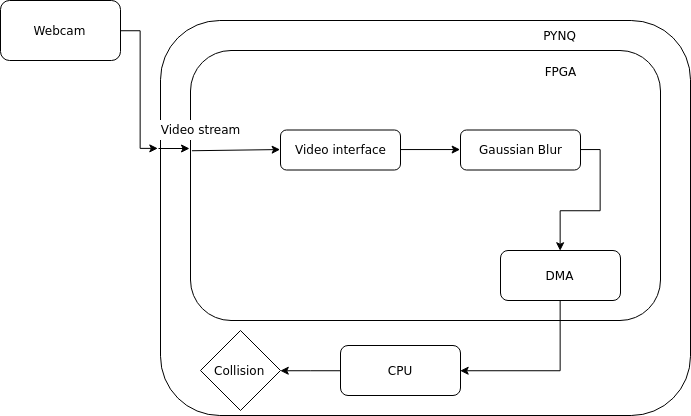
\includegraphics[scale=0.4]{Images/PipielineFinalFinal-Page-1.png}
    \caption{Final FPGA design overview}
    \label{fig:fpga1}
\end{figure}

\begin{figure}
    \centering
    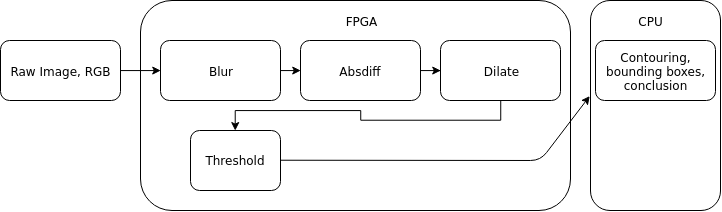
\includegraphics[scale=0.4]{Images/PipielineFinalFinal-Page-2.png}
    \caption{Intended accelerator overview}
    \label{fig:fpga2}
\end{figure}

The Gaussian Blur accelerator is modelled after \cite{cong2014optimal} and looks like figure [\ref{fig:pipeline-overview}].

\subsection{Accelerator pipeline}
The accelerator's pipeline follows a sequential pattern [\ref{fig:Real_Pipe}], meaning the pixels are inputted from left to right, top to bottom. The reason for this is avoiding unnecessary complexity, since the intended camera model outputs the pixel-values in this fashion. Another reason is that this method is able to get the throughput needed, it has the least amount of latency, and uses the least amount of resources.

The alternative method to a sequential pipeline would be a way to partly load pixel-values vertically, instead of horizontally. Figure \ref{fig:Alt_Pipe} shows this pattern. This, however, makes no sense without hardware support, which the camera does not have. If the camera would be able to output pixels in chunks equal to the Gaussian Blur kernel, it would make sense to use this, to lower the latency from the Gaussian Blur filter.
\begin{figure}
    \centering
    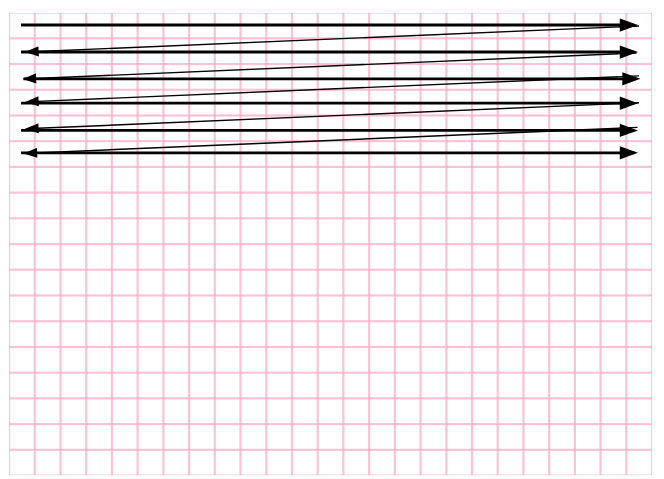
\includegraphics[scale=0.4]{Images/real_pipeline.png}
    \caption{Real pipeline}
    \label{fig:Real_Pipe}
\end{figure}

\begin{figure}
    \centering
    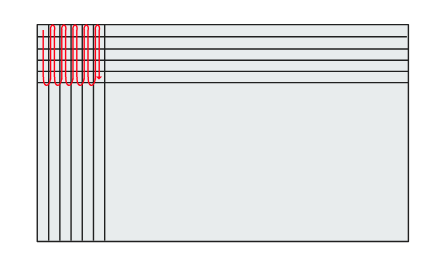
\includegraphics[scale=0.75]{Images/alternative_pipline.png}
    \caption{Alternative pipeline}
    \label{fig:Alt_Pipe}
\end{figure}

\subsubsection{Video interface}
The video interface receives signals from the camera module and produces a stream of pixels. The communication between the camera and the video interface is clocked by the pixel clock from the camera. A vertical synchronization 
signal signifies the end of a frame and the start of a new frame. The href signal signifies that the 8-bit data bus is currently holding valid pixel data. Using these signals and the data bus, the video interface reads image frames from the camera module.

As the camera module was abandoned due to difficulties configuring it, the video interface is not used in the final product.

\subsubsection{Grayscale}
The grayscale component is the first step of the pipeline after pixel values are sent from the data source. It grayscales an image with the following equation:

\begin{equation}
    o = r \times 0.3 + g \times 0.59 + b \times 0.11
\end{equation}

where $r$, $g$ and $b$ are the respective RGB channel values and $o$ is the output, namely the resulting grayscaled value.

It incrementally produces this sum, outputting the grayscaled value when the blue value arrives, then resets and starts over again with the next pixel. This ensures that the grayscale only has 3 clock-cycles of latency, and a throughput of one third of the input, meaning no data is lost.

This module is not used in the final product, as converting the image to grayscale before piping the data to the PYNQ saved two thirds of the bandwidth used over the network interface.

\subsubsection{Gaussian blur}
The Gaussian blur part of the accelerator takes grayscaled values as input and blurs them using a computational kernel. Because Gaussian blur needs to calculate the resulting pixel value from pixels directly adjacent to it, it is necessary to store the pixels for later use. This is done by creating a series of queues, as outlined in Figure \ref{fig:gauss}, and outputting the correct values through the filter kernel.

\subsubsection{Absdiff}
Absdiff is utilized to find the absolute difference in value between the same pixel from consecutive images. The module takes grayscale-values as input, and outputs the absolute difference.

It does this by inserting all values of the current frame into a queue. The next input value will then be the first value of the next frame, and the absolute difference between them is output by the module.

Due to unresolved bugs, this module was not incorporated in the final design.

\subsubsection{Threshold}
Threshold is used to filter out any noise from the Absdiff by creating a binary image. Small values from Absdiff are more likely to come from random noise than from an actual object moving in the picture.

Threshold is implemented by checking the input values, and output a value of 255 if it exceeds the threshold, and a value of 0 if it does not exceed it.

This module was also not used in the final design, as the module directly before it was excluded from the design.

\subsubsection{Dilate}
Dilation is an image filtering operation where in a given area on the image the maximum value is chosen and replaces the center value in the chosen area. This module was implemented, tested and was proven functional, however including it in the final design was deemed impractical, due to its position in the pipeline. 
\subsubsection{DMA}
When the Gaussian blur component is finished doing its work, the pixel values are passed in to the DMA for fast transfer into DDR memory and direct access by the CPU.
The DMA module is an IP block provided by the Vivado IP library.


\subsection{The PYNQ CPU}
The Cortex-A9 CPU is used on the PYNQ to further process the images from the FPGA. The CPU runs Python code that reads images from memory and calculates whether there is an incoming object or not. The images which are read from memory have been pre-processed by the custom accelerator for the CPU to work with. The images are already grayscaled and Gaussian blurred to make it easier to detect movement. The algorithm for the detection of incoming objects works as follows:

\begin{enumerate}
    \item Two pre-processed images from the camera are compared to each other to find out where something has been moving
    \item The size of the area that has been changed is calculated and stored. 
    \item When a new image is received in the next frame, the processor can determine if the new area that is changed is bigger or smaller than the previously stored value. If the area is bigger something is incoming.
\end{enumerate}

OpenCV is utilized to perform these calculations. When an incoming object is detected, a signal is sent to the MCU through a 3-bit data bus to the PCB. These lines transmit a value ranging from 0 to 7 indicating the estimated probability of a collision.

\subsection{The Microprocessor}
% Stats
\subsubsection{Specification} % Title pending
The EFM32GG980F1024-QFP100 was selected to be the PCB's MCU because of its flexibility and feature-richness. This made it possible to progress quickly on other parts of the design, before the exact details of its operation were decided upon. The chips most important qualities for this project were:
%TODO: Reasons why these are important? 
\begin{itemize}
    \item Comparatively high processing power
    \item Support for a number of protocols such as UART, USART and USB 
    \item Familiarity to group members
    \item QFP100 14x14mm package (simpler to solder than alternatives) %Non-solder-hell
\end{itemize}

\subsubsection{Device Communication}
See \autoref{fig:PCB_COMM}.
\begin{figure}
    \centering
    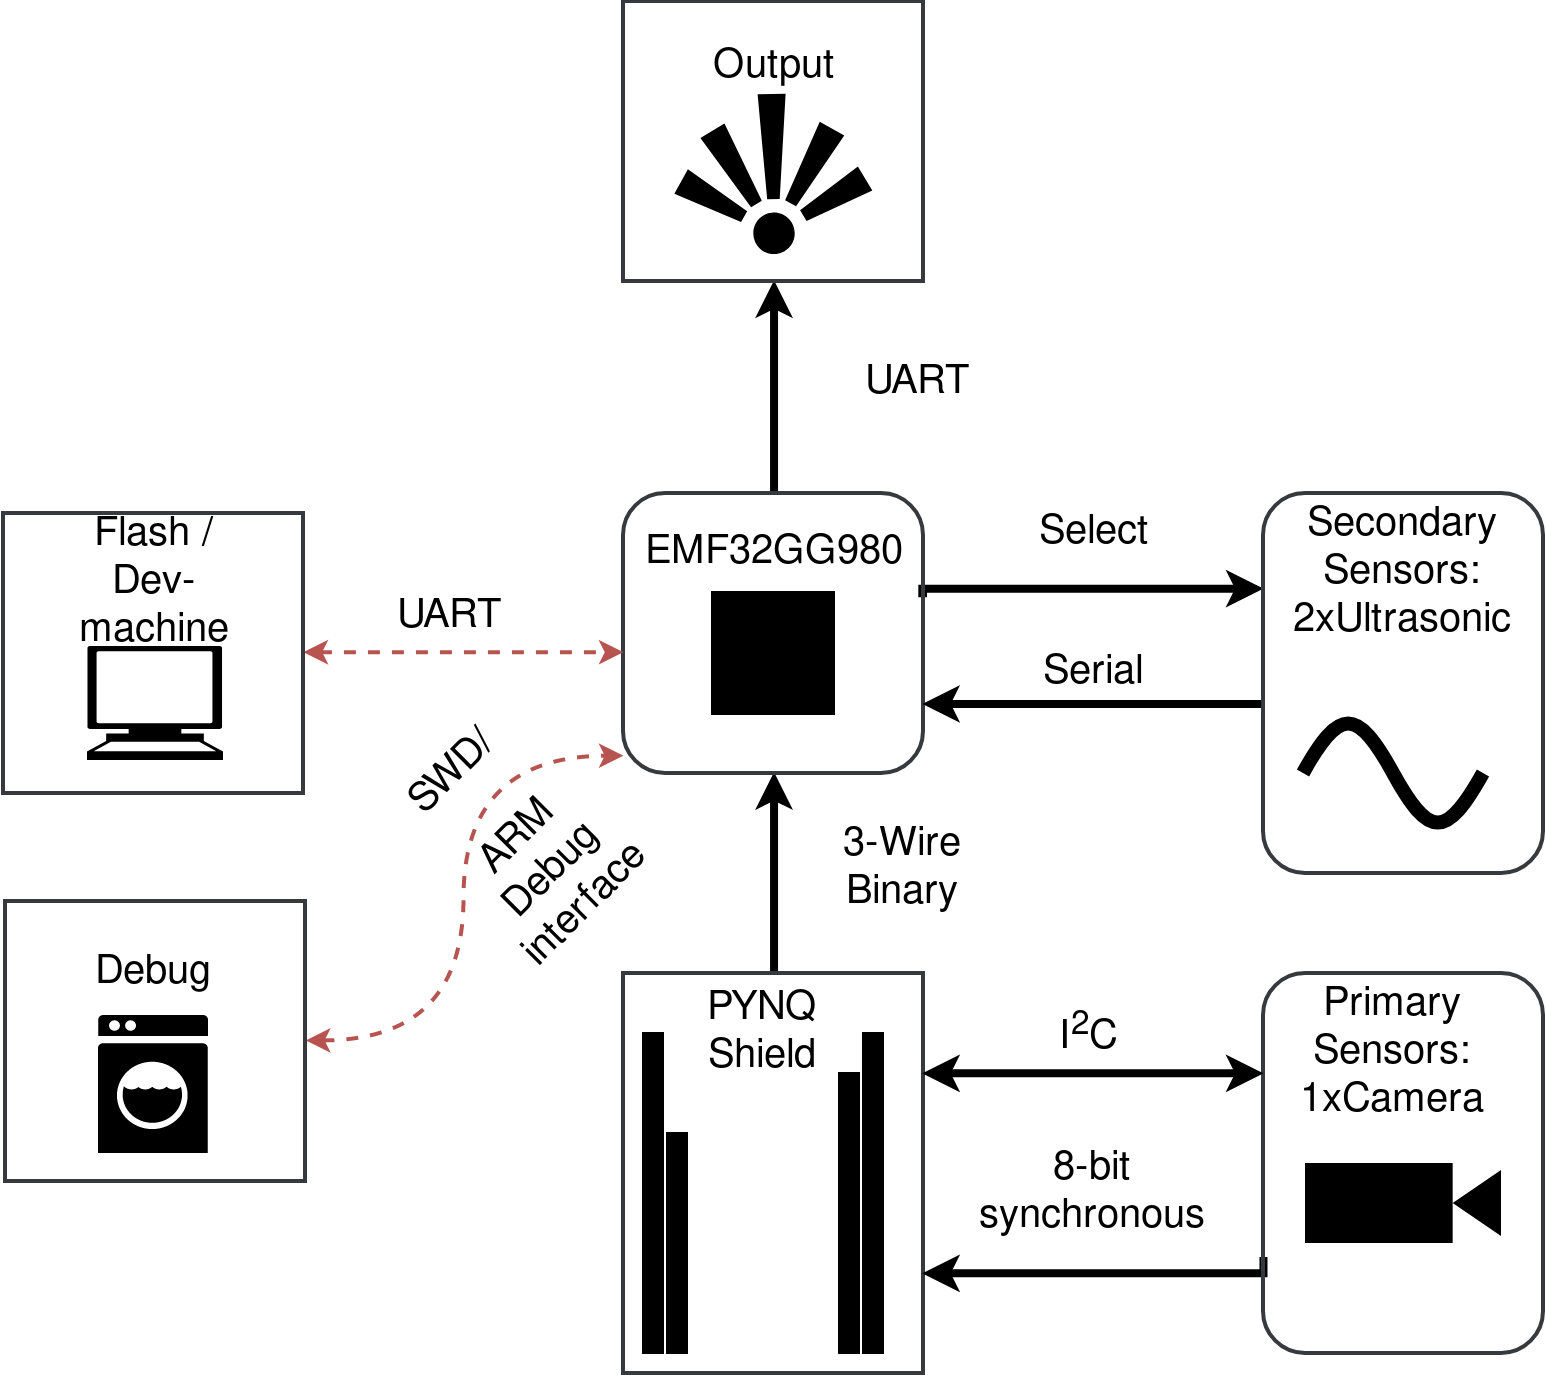
\includegraphics[scale=0.2]{Images/PCB(7).png}
    \caption{Communication on the BRICOLEUR PCB}
    \label{fig:PCB_COMM}
\end{figure}

\subsubsection{Ultrasonic analysis}

Each of the ultrasonic sensors will detect a different distance to an object. This difference can be used to calculate the position of the object relative to the sensors with a technique known as trilateration:

\begin{itemize}
    \item Let each sensor be the center of a circle, and let the distance to the object be the radius of the circle. Then the position of the object may be found by calculating the intersection of the circles. This is illustrated in Figure \ref{fig:ultrasonic_trilateration}.
    \item Please note that for two circles there will be two solutions, but one of these solutions will be behind the sensors, and can therefore be ignored.
    \item Also note that two circles will only give a 2D position, but this is sufficient to meet the assumption of an object moving along the ground. If the system should be expanded to handle objects thrown through the air, there would be a need for three sensors in order to find the 3D intersection point of three spheres. This would have four solutions, but only one of the solutions would be both in front of the sensors and above the ground.
    \item Once the position of the object at a given time is found, it is possible to measure the change in position over time. These positions can then be used to estimate velocity and interpolate a line, which in turn can used to estimate the future position of the object. This is illustrated in Figure \ref{fig:ultrasonic_motion}.
    \item By looking at where the object will intersect the x-axis (the system is at $y = 0$), one can conclude whether the object will collide heads-on, hit the edge of our system, or misses it completely. This means that even if an object is moving toward the sensors, it is possible to detect that it will actually miss the system.
\end{itemize}

\begin{figure}[h]
    \centering
    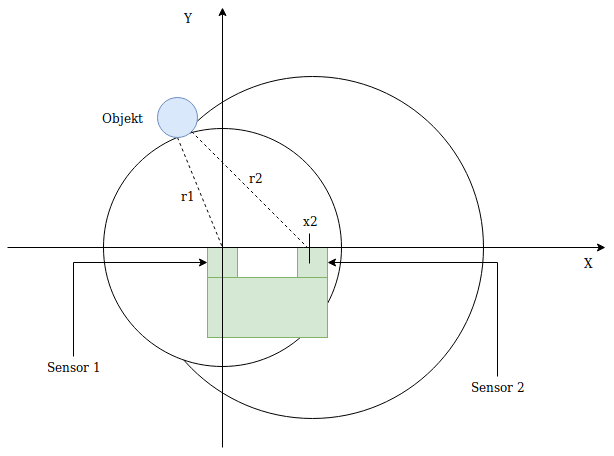
\includegraphics[scale=0.5]{Images/ultrasonic_trilateration.png}
    \caption{Ultrasonic: The difference in distance is used to find the position of the object}
    \label{fig:ultrasonic_trilateration}
\end{figure}

\begin{figure}
    \centering
    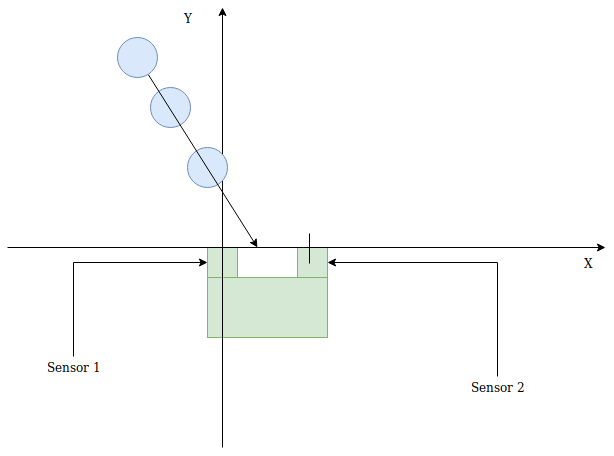
\includegraphics[scale=0.5]{Images/ultrasonic_motion.png}
    \caption{Ultrasonic: The different positions over time are used to estimate the future position of the object}
    \label{fig:ultrasonic_motion}
\end{figure}

% How do we determine what to output 
\subsubsection{Combining the conclusions from the camera and ultrasonic sensors}

Both the camera system and the ultrasonic system output a probability of collision. In order to combine these conclusions, we have to take into account that the delay of the systems might be different. If we simply take a (weighted) average, we could risk that one of the systems output a high probability while the other outputs a low probability, and shortly after the opposite happens. This would then only lead to a medium value, even if both the systems report a high probability of collision, just with a delay between them.

Because of this, we simply take the maximum value of the two conclusions, which ensures that the final conclusion is not lower than it should be.

\subsection{The PCB}

\begin{wrapfigure}{R}{0.4\textwidth}
    \centering
    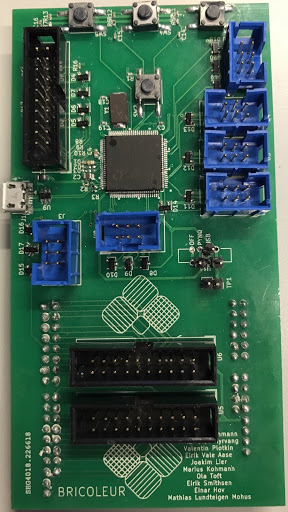
\includegraphics[scale=0.4]{Images/PCB_bricoleur.jpg}
    \caption{Assembled PCB}
    \label{fig:pcb}
\end{wrapfigure}

In order to cleanly connect the project's various components, a custom PCB was designed. The design behind the BRICOLEUR PCB was inspired by SiliconLabs' STK3700 board, in part because of the similar MCUs. Schematics and a complete list of components can be found in appendix A: Schematics and B: Components.


\subsubsection{Features}
\begin{itemize}
    \item Three switchable power sources: USB, PYNQ and external.
    \item J-Link compatible debug header
    \item Two camera headers 
    \item Three ultrasonic sensor connectors
    \item Header for UART-based bootloader communication
    \item Two UART/USART compatible input/output headers
    \item Arduino-compatible main header
    \item ESD protection on all inputs
    \item Debug LEDs and buttons
\end{itemize}

\subsubsection{Design}
The PCB was designed to be in accordance with Silicon Labs' application notes. The following documents were found to be of particular relevance:
\begin{itemize}
    \item AN0002 - Hardware Design considerations
    \item AN0003 - UART Bootloader
    \item AN0042 - USB/UART Bootloader
    \item AN0046 - USB Hardware Design Guide
\end{itemize}
% TODO: Noen jeg har glemt?

\subsubsection{Power supply}
The BRICOLEUR PCB is designed to operate at 3.3V. Other voltages are not officially supported, and all parts connected to the board are expected to operate at this voltage level. Power may be supplied to the board and its components in three ways: 

%Fuckings fuckleaf dont like enumeration with wrappings, pathetic
\begin{enumerate}
    \item USB: A microUSB cable can be connected directly to the board from a power supplying USB device. The MCU's internal voltage regulator converts the USB standard's 5V to 3.3V, which is then output on all power lines. Note that the PCB will not be able to power other devices through USB, even if it is provided power from another source. 
    \item PYNQ: The PYNQ Z1 Arduino Uno-style header contains a power pin which can output 3.3V directly to the PCB. This is expected to be the main mode of operation for the system.
    \item Header: A dedicated power pin has been exposed. It is intended primarily for debugging and as a backup. This point of entry has no safeguards: Be careful to ONLY apply 3.3V. 
\end{enumerate}

\subsubsection{PCB bricolage}
Shortly after placing the PCB order it was discovered that the way in which the ultrasonic sensors were connected would require some additional hardware, namely diodes. The reason for this was the pin-saving way in which the sensor outputs were wired. Since each ultrasonic sensor would be polled in order, out of fear for interference, it was thought that they could safely share a single MCU input pin. However, this opened up for the possibility that the high signal from one sensor could be sent to another sensor whose pin was currently driven low, causing a short circuit. Diodes solve this issue by  limiting the current direction. Because the board had no additional space for diodes, the cables were instead selected to be their mounting point.

Additionally, it turns out that the footprint intended for the power switch was poorly dimensioned. This has been amended by replacing the switch with a set of header pins and an externally wired power switch. A jumper between the correct pins can perform the switch's duty as well. 

\begin{figure}
    \centering
    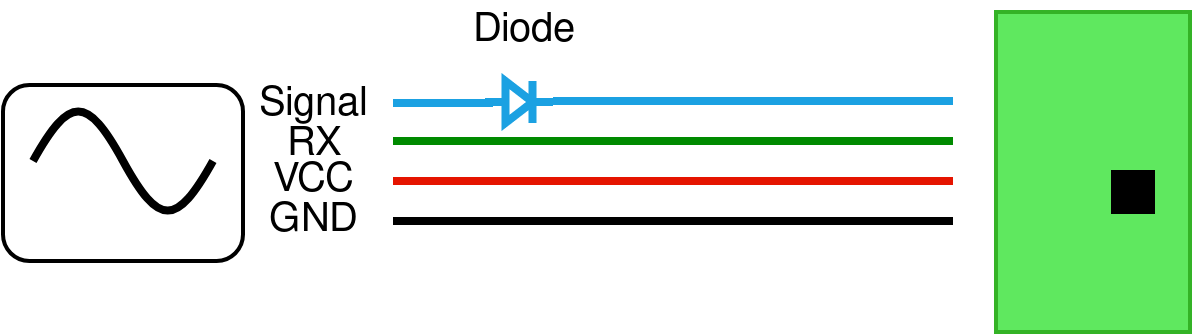
\includegraphics[scale=0.25]{Images/Cable.png}
    \caption{The cables connecting the ultrasonic sensors to the PCB}
    \label{fig:cable}
\end{figure}